\chapter{Introduction To Convolutional Neural Networks}
The Convolutional Neural Network (CNN) is a well-known deep learning architecture that was loosely inspired by the natural visual perception mechanism of some living organisms.
This comes from a paper by Hubel and Wiesel \cite{hubel1968receptive} in 1959 where they found that their were specific cells in the visual cortex of animals that were responsible for detecting light in the receptive field, which eventually won them a Nobel Prize. 
It was not until 1990 that LeCun et al. \cite{lecun1990handwritten} released the crucial paper that would establish modern framework for CNNs. 
Their model was a multiple layer neural network called LeNet-5 that could classify 28x28 greyscale hand written digit images with very high accuracy. 
As seen in Fig.~\ref{f:lenet} LeNet-5 has multiple layers and can be trained with the back-propagation algorithm \cite{hecht1988theory}, but used a low number of parameter values for its size. 
To achieve this LeNet-5 used two core components, which we will discuss in the next section.

\begin{figure}[h!]
	\centering
		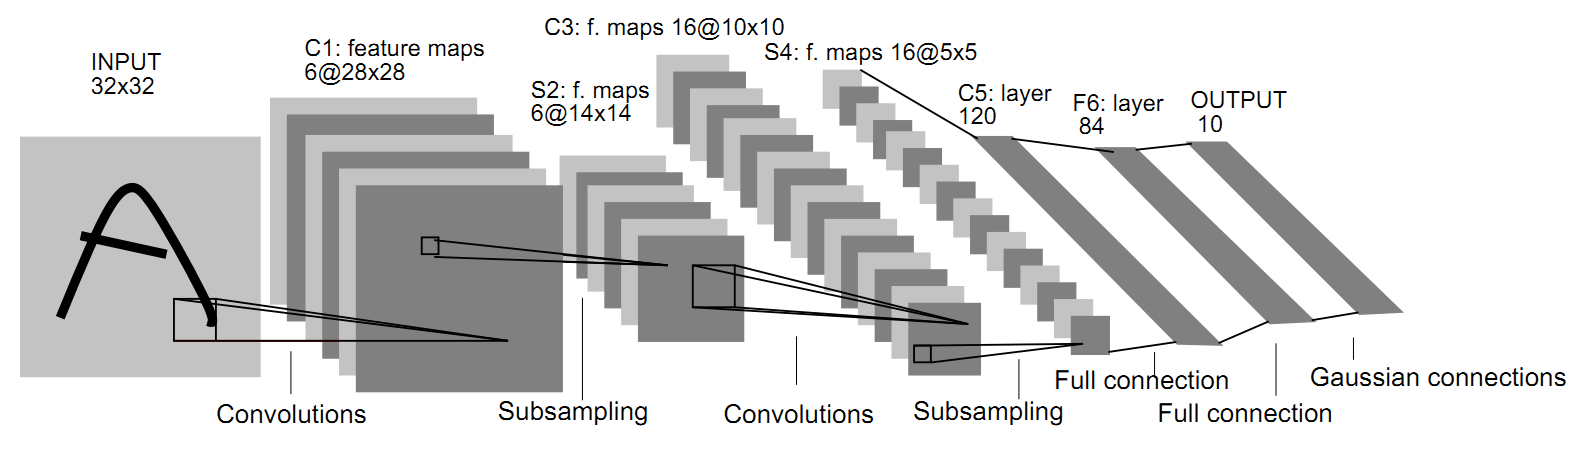
\includegraphics[width=0.95\textwidth]{figures/lenet5.png}
	\caption{The architecture for LeNet-5, which is composed of repeating convolution and pooling layers.}
	\label{f:lenet}
\end{figure}

\section{Basic CNN Components}
While there are many different layer types in current literature, here we will focus on the two introduced in LeNet-5, which are still used today along with some variants of them. 

\subsection{Convolutional Layer}
The first is the convolution layer. 
Its purpose is to learn feature representations of the inputs. 
Each convolution layer has a specified number of kernels where each kernel is unique as to generate a distinct feature map. 
Each neuron of a feature map is connected to a region of neighboring neurons in the previous layer. 
The size of the connection is known as the kernel size or the receptive field size. 
The feature map is obtained by first convolving the input with the kernel and then applying an element-wise nonlinear activation function on the result. 
Because it is a convolution operation each kernel is shared with all spatial locations of the input. 
This spatial weight sharing is what creates the low parameter number compared to a regular neural network which fully connects all inputs and outputs. 
It also allows the CNN to take advantage of the underlying structure in images. 
Topological information, i.e., spatial information about the structure in an image, such as adjacency and rotations are also taken into account. 
The equation for finding the feature value at location $(i,j)$ in the $k^{th}$ feature map of the $l^{th}$ layer, $z^l_{i,j,k}$ is
\begin{equation}
z^l_{i,j,k} = {\textbf{w}^l_k}^T \textbf{x}^l_{i,j} + b^l_k
\label{eq:convbasic}
\end{equation}
where $\textbf{w}^l_k$ and $b^l_k$ are the weight vector, or convolution kernel, and the bias term of the $l^{th}$ layer respectively, and $\textbf{x}^l_{i,j}$ is the input patch centered at location $(i,j)$ of the $l^{th}$ layer. 
An example of this operation can be seen in Fig.~\ref{f:convolution}. 
After the convolution is applied the result is then put through the nonlinear activation function:
\begin{equation}
a^l_{i,j,k} = a(z^l_{i,j,k})
\label{eq:activationbasic}
\end{equation}
where $a(\cdot)$ is the nonlinear activation function. 
We will discuss different activation functions in great detail in Chapter \ref{StateOfTheArt}.

\begin{figure}[h!]
	\centering
		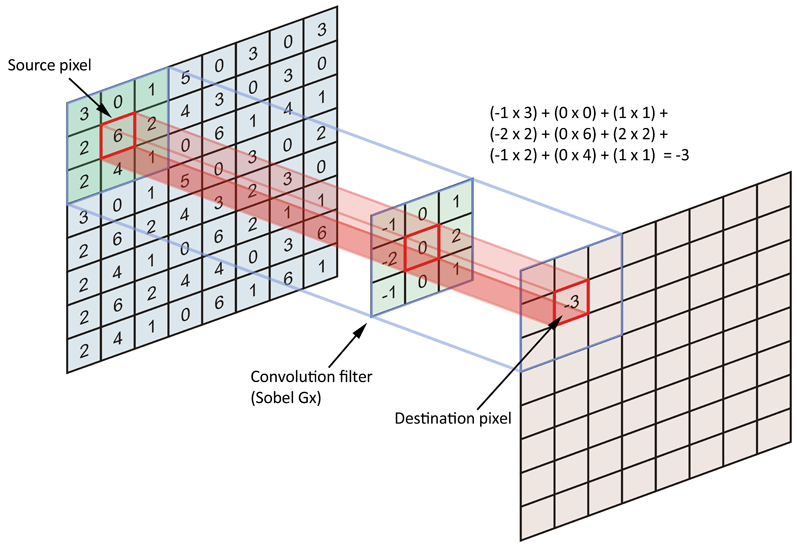
\includegraphics[width=0.95\textwidth]{figures/convolution.png}
	\caption{Convolution operation performed on a single feature location and one convolution kernel \cite{convolution}.}
	\label{f:convolution}
\end{figure}


\subsection{Pooling Layer}
The other key layer is the pooling layer shown in Fig.\ref{f:lenet} as subsampling. 
The pooling layer comes after a convolution layer and it performs a reduction in the resolution of the feature map. 
This layer works typically with two arguments: the spatial size of the pooling window $F$ and the stride, or shift per operation, $S$.
It is accomplished in a similar manner to convolution, starting at the top right a window of size $F \times F$ is grabbed.
From this window the pooling function is used, which is commonly a \textbf{MAX} function.
The window then moves over by $S$ pixels and the above operation happens again.
This is repeated until the whole image is covered.
For example, if one chooses $F = 2$ and $S = 2$ they will be selecting the maximum pixel in a $2 \times 2$ window and moving 2 pixels over exactly as shown in Fig.~\ref{f:maxpool}.
Note that this reduces the original image by a factor of $F = 2$.
This serves the purpose of reducing the number of multiplications the architecture must perform and also aims to achieve shift invariance. 
We will discuss different pooling techniques in Chapter \ref{StateOfTheArt}.

\begin{figure}[h!]
	\centering
		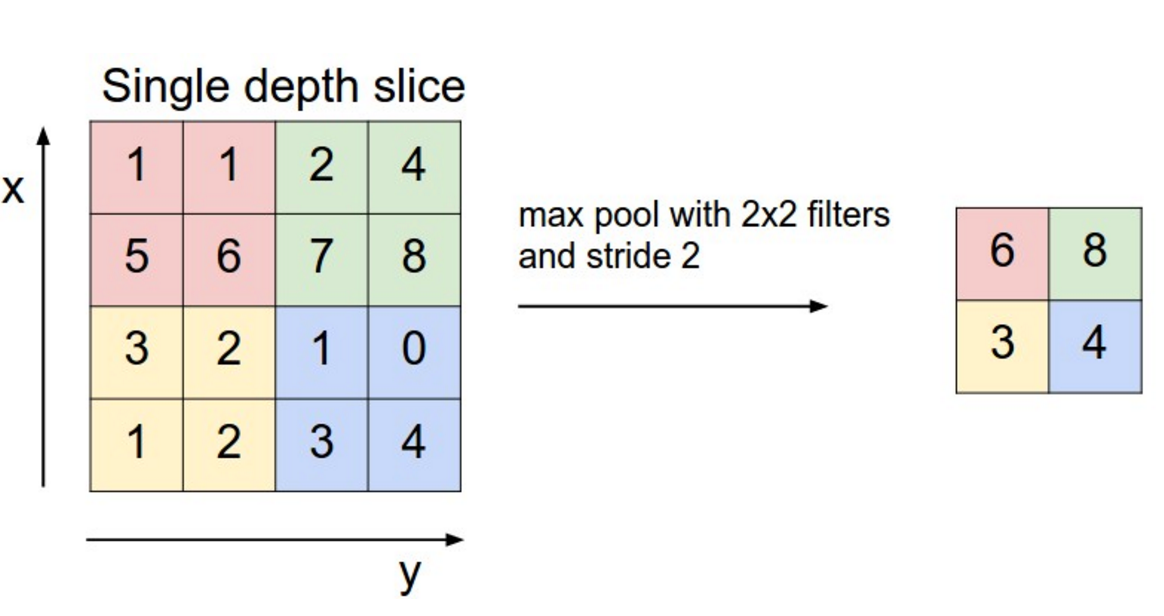
\includegraphics[width=0.95\textwidth]{figures/maxpool.png}
	\caption{Example max pooling operation with a size of 2x2. A 2x2 window is moved over the input with a stride of 2 and the maximum value of the window is taken \cite{maxpooling}.}
	\label{f:maxpool}
\end{figure}

There is also the inverse of pooling, often called upsampling, that will increase the resolution of the feature maps.
There are several cases where this is a desired effect which we will discuss later.


\subsection{CNN Common Tasks}
The last layers of LeNet-5 are fully connected layers like that of a regular Feed-Forward Neural Network (FNN), sometimes called Multilayer Perceptrons \cite{rumelhart1985learning}. 
The second to last layer is sometimes called a decision layer as it takes the outputs from the feature mapping and combines them together. 
The last layer is a fully connected layer of size 10, which corresponds to the number of classes in that particular data set. 
The classes, which are digits numbered 0 through 9, are represented as a `one hot' vector, meaning that if the class is the digit `0' the first element of the output vector should be 1 and the rest should be 0. 
This can be thought of as a probability distribution on the classes. 
This is an important representation because it allows one to use loss functions that minimizes the differences of distributions opening up many potential loss functions.
This was the common use case for CNNs for a while, given an image predict a distribution over a set of classes. 
This task is known as \textit{classification}. 

Recently CNNs have seen use in another area known as \textit{semantic segmentation}.
Semantic segmentation, also sometimes just called segmentation, is the process of partitioning an image into multiple segments, or sets of pixels. 
More precisely, segmentation is the process of assigning a class from our classification set to each pixel, or potentially area of pixels, in an image. 
Unlike classification, the output of this CNN would typically be in the form of an image.
Typically the network will output a distribution over a set of classes \textit{per pixel} and then the pixel is labeled with the class with the highest probability. 
There are many applications where image classification alone does not giving enough information and one needs pixel-level labels. 
Examples include: detecting road signs \cite{maldonado2007road}, detecting tumors in medical imaging \cite{li2015automatic, lyksborg2015ensemble, kainz2015semantic, havaei2017brain}, detecting objects of interest from satellite photos \cite{chen2013vehicle}, finding pedestrians \cite{du2016fused}, and many more. 
Having pixel level labels allows multiple objects of different classes to be detected in one image compared to image level labels where there is a single output per image.

In recent years, CNNs have obtained state of the art results on almost all classification and segmentation data sets. 
The improvements in CNNs have come from a few different areas including better computers, improvements to initialization of network weights, and specific architectures to combat problem areas of deep networks. 
In this next chapter we will go through a list of improvements and key papers.  